\documentclass[portuguese]{textolivre}

% metadata
\journalname{Texto Livre}
\thevolume{17}
%\thenumber{1} % old template
\theyear{2024}
\receiveddate{\DTMdisplaydate{2024}{2}{14}{-1}}
\accepteddate{\DTMdisplaydate{2024}{3}{14}{-1}}
\publisheddate{\DTMdisplaydate{2024}{4}{22}{-1}}
\corrauthor{Luciano Magnoni Tocaia}
\articledoi{10.1590/1983-3652.2024.51248}
%\articleid{NNNN} % if the article ID is not the last 5 numbers of its DOI, provide it using \articleid{} commmand 
% list of available sesscions in the journal: articles, dossier, reports, essays, reviews, interviews, editorial
\articlesessionname{articles}
\runningauthor{Tocaia}
%\editorname{Leonardo Araújo} % old template
\sectioneditorname{Daniervelin Pereira}
\layouteditorname{João Mesquita}

\title{Planejamento e elaboração de atividades didáticas para o ensino de francês em um ambiente virtual de aprendizagem: ensino de gêneros textuais e desenvolvimento de capacidades de linguagem}
\othertitle{Planning and developing didactic activities for teaching French in a virtual learning environment: teaching textual genres and developing language capacities}

\author[1]{Luciano Magnoni Tocaia~\orcid{0000-0002-1259-2045}\thanks{Email: \href{mailto:lucianotocaia@uol.com.br}{lucianotocaia@uol.com.br}}}
\affil[1]{Universidade Federal de Minas Gerais, Faculdade de Letras, Belo Horizonte, MG, Brasil.}

\usepackage{enumerate}
\usepackage[inline]{enumitem}
\usepackage{array}

\addbibresource{article.bib}

\begin{document}
\maketitle
\begin{polyabstract}
\begin{abstract}
Este artigo tem por objetivo apresentar um relato de experiência sobre o processo de elaboração de material didático para um curso online destinado ao ensino de francês como língua estrangeira por meio do ambiente virtual de aprendizagem Moodle. O curso, de natureza assíncrona, foi desenvolvido no quadro de uma formação pedagógica e linguística para estagiários de francês e teve a participação de dois alunos-estagiários bolsistas em um centro de extensão de uma universidade federal brasileira. O curso baseia-se nos pressupostos teórico-metodológicos propostos pelo Interacionismo Sociodiscursivo \cite{bronckart_atividade_1999,bronckart_teorias_2021} e no uso de gêneros textuais para o ensino-aprendizagem de línguas estrangeiras \cite{dolz_pour_1998,schneuwly_generos_2004}. O material desenvolvido foi organizado de forma a desenvolver atividades na plataforma Moodle que visam tanto a sensibilizar ao aprendizado do francês por meio dos gêneros textuais quanto a contribuir para o desenvolvimento de capacidades de linguagem \cite{schneuwly_generos_2004,stutz_construcao_2011} dos alunos, possivelmente transferíveis a outros gêneros. Os resultados, após a elaboração do curso, apontam para a eficácia do ambiente virtual Moodle para o ensino de línguas e o respectivo desenvolvimento de atividades interacionais que possibilitam o agir em língua estrangeira, em virtude da variedade de recursos oferecidos pela plataforma, podendo atender a demandas e a estilos diversos de aprendizagem.

\keywords{Gêneros textuais \sep Capacidades de linguagem \sep Ambiente virtual Moodle \sep Francês língua estrangeira}
\end{abstract}

\begin{english}
\begin{abstract}
The aim of this article is to present and describe part of the process of developing didactic material for an online course aimed at teaching French as a foreign language using the Moodle virtual environment. The asynchronous course was developed over the course of a year as part of a pedagogical and linguistic training program for French trainees, with the participation of two trainee students from an extension center at a Brazilian federal university. To this end, the research is based on the theoretical-methodological framework of Sociodiscursive Interactionism \cite{bronckart_atividade_1999,bronckart_teorias_2021} and especially regarding the use of textual genres in the teaching and learning of languages \cite{dolz_pour_1998,schneuwly_generos_2004}. The material proposes activities on the Moodle platform aimed at contributing to the development of students' language capacities \cite{schneuwly_generos_2004,stutz_construcao_2011}, possibly transferable to other genres. The results point to the effectiveness of the Moodle virtual environment for language teaching and the respective development of interactional activities that make it possible to act in a foreign language, due to the variety of resources offered by the platform, which can meet the demands and diverse learning styles.

\keywords{Textual genres \sep Language capacities \sep Moodle virtual learning environment \sep French as a foreign language}
\end{abstract}
\end{english}
\end{polyabstract}

\section{Introduction}\label{sec-intro}
The educational context is seen as a social ecosystem, exhibiting characteristics of a complex adaptive system, composed of nested systems, such as schools, classrooms, families, and so on. Agents within these systems, such as educators, students, and teachers contribute to the emerging dynamics of their relationships within these systems. An investigation of ecological systems requires lenses that contemplate the possible relationships and dynamics among their agents. The ecological approach is considered a way of thinking and studying organisms in their relationship with the environment. \textcite{vanlier2004} reminds us that this approach is based on systems theory, complexity theory, chaos theory, and cybernetics, recognizing the complexity and interrelationship of the processes that lead to the creation of an environment.


Underpinned by the construct of ecological perspective and coupled with the concept of affordance, this study attempts to better understand how pre-service teachers exercise their agency using mobile digital technologies. The concept of affordance can serve to identify actions arising from these teachers’perceptions. Moreover, we resort to discussions on agency as a complex system in Applied Linguistics \cite{mercer2012, larsen2019} because they can advance our understanding of patterns that emerge from the perception-action relations as these pre-service teachers exercise agency.


The concept of agency is present in discussions of several areas of knowledge and has been on the agenda of Applied Linguistics. Discussions by \textcite{vanlier2004,vanlier2010a,mercer2011,mercer2012,mercer2018,larsen2019}, however, stand out from those of other scholars because they rely on the ecological perspective and complexity theory.


Although the field of Applied Linguistics is not devoid of discussions on these perspectives, the dimensions of pre-service teachers’ exercise of agency mediated by mobile digital technologies have been underexplored, which justifies the development of this study. With that in mind, we seek to identify: 

\begin{enumerate*}[label=\roman*)]
	\item Instances of the agency exercised by pre-service teachers;
	\item Actions mediated by the use of cell phones by these teachers;
	\item Intrapersonal issues (emotions, beliefs, motivation, etc.) that can influence their agency.
\end{enumerate*}


We briefly present the theories and concepts undergirding this study, namely: the ecological approach, complexity theory, mobile learning, and agency.


\section{A plataforma Moodle como ambiente virtual para o ensino de línguas}\label{sec-aplataformamoodlecomoambientevirtualparaoensinodelínguas}

Nas duas últimas décadas, percebemos um grande aumento da oferta de
cursos para o ensino de idiomas oferecidos em ambientes virtuais, seja
na modalidade síncrona, seja na modalidade assíncrona. Nesses cursos, os
processos de interação entre o professor/aluno e entre o aluno/conteúdo
proposto para o aprendizado de determinado idioma acontecem por meio de
ambientes virtuais de aprendizagem (AVA), que assumem um papel central
no que diz respeito à participação e ao aproveitamento do curso pelos
alunos e no processo de ensino-aprendizagem efetuado pelos professores.
De acordo com \textcite{lima_https://proceedings.science/isa-2017/trabalhos/metodos-mais-usados-para-avaliacoes--ambientes-virtuais--aprendizagem-avas_2018}, num AVA, o aluno inscrito em um curso tem acesso a múltiplos recursos de interação, ou seja, suportes necessários para o aprendizado à distância, como, por exemplo, chats, fóruns, aulas interativas, questionários, glossários, vídeos, entre outros, o que faz do professor um mediador do conhecimento entre o aluno inscrito no curso e os conteúdos ministrados. Além de propiciarem aos alunos uma forma mais ativa de lidar com seu aprendizado, permitindo uma melhor organização e a oportunidade do autoestudo, um AVA funciona, nos cursos síncronos e assíncronos, como a verdadeira sala de aula, porém, virtualizada. Para \textcite{bersch_moodle_2009}, os AVA buscam facilitar esse processo ao reunirem um conjunto de ferramentas que permite disponibilizar materiais diversificados, propor, realizar e avaliar diferentes tipos de atividades.

No caso do curso que descreveremos, o AVA escolhido para hospedar os
cursos de idiomas foi o Moodle (\emph{Modular Object-Oriented Dynamic
	Learning Environment}), desenvolvido por Martin Dougiamas. Trata-se de
uma ferramenta livre e de código aberto, muito utilizada pelas
instituições de ensino públicas e particulares, que foi desenvolvida
para propiciar a professores e alunos um sistema seguro e totalmente
integrado, que tem por objetivo criar ambientes de aprendizagem
personalizados, como explicam as palavras de \textcite[p. 31]{gervasio_nvestigacao_2019}:
\enquote{[$\ldots$] é inegável que o Moodle se tornou uma poderosa ferramenta
tanto para o ensino EAD como no presencial, sua variedade de plugins e
flexibilidade de customização o torna utilizável em qualquer curso e
modalidade de ensino}. Ainda, segundo o pesquisador, \enquote{a combinação de
metodologias de ensino, agrupadas pelas tecnologias disponíveis no
ambiente, é fundamental para o design de cursos direcionados
especificamente a área de atuação}. \cite[p. 31]{gervasio_nvestigacao_2019}.

De acordo com \textcite{thomaz_principios_2022}, a plataforma Moodle foi desenvolvida a partir de quatro princípios, o Construtivismo, o Construtivismo Social, o Construcionismo e o Comportamento Conectado e Separado, visto que a
interação social (a ação), por meio da linguagem, permite o
estabelecimento de uma corrente colaborativa em permanente comunicação,
síncrona e assíncrona, colhendo frutos para um aprendizado de cunho
social, histórico e cultural, que se define por novas formas autônomas
de aprender crítica e dinamicamente, construir ideias, comunicar e se
informar. Embora dependa de uma prática pedagógica igualmente
interacionista, a plataforma Moodle busca valorizar o processo de
aprendizagem ao disponibilizar um rol de ferramentas interativas de
diferentes qualidades que oferecem ao usuário a possibilidade de
construção de significados ao efetivarem as variadas propostas de
interação, negociação e construção colaborativa de conhecimento
disponíveis. Na \Cref{tab-01}, reproduzimos uma lista de ferramentas encontradas no AVA Moodle, elaborada por \textcite{mayrink_ensino_2017}, com
base em estudos de \textcite{valente_educacao_2011}, que ilustra a forma como vários desses recursos podem ser agrupados e utilizados para o desenvolvimento
de atividades didáticas em cursos de idiomas.

\begin{table}[h!]
\centering \small
\begin{threeparttable}
\caption{Agrupamento de ferramentas da Plataforma Moodle.}
\label{tab-01}
\begin{tabular}{>{\raggedright\arraybackslash}p{3cm} >{\raggedright\arraybackslash}p{3cm} >{\raggedright\arraybackslash}p{6cm}}
\toprule
Potencial de interatividade & Recurso & Tipo de atividade \\
\midrule
Baixo potencial de interatividade (aluno-máquina- conteúdo) &
\begin{minipage}[t]{\linewidth}
\begin{itemize}[leftmargin=*,topsep=-0pt,partopsep=0pt,parsep=0pt,itemsep=0pt]
    \item Questionário
    \item Escolha
    \item Pergunta
\end{itemize} 
\end{minipage}
&
\begin{minipage}[t]{\linewidth}
\begin{itemize}[leftmargin=*,topsep=-0pt,partopsep=0pt,parsep=0pt,itemsep=0pt]
    \item Completar frases, diálogos, canções, textos (com espaço ou close). 
    \item Ordenar um diálogo ou texto.
    \item Organizar o vocabulário em diferentes campos semânticos.
    \item Relacionar ou preencher colunas.
    \item Relacionar imagens a palavras/textos.
    \item Escolher a alternativa correta.
\end{itemize} 
\end{minipage}
\\
Potencial de interatividade médio (aluno-máquina-conteúdo-professor) &
\begin{minipage}[t]{\linewidth}
\begin{itemize}[leftmargin=*,topsep=-0pt,partopsep=0pt,parsep=0pt,itemsep=0pt]
    \item Tarefa
\end{itemize} 
\end{minipage}
&
\begin{minipage}[t]{\linewidth}
\begin{itemize}[leftmargin=*,topsep=-0pt,partopsep=0pt,parsep=0pt,itemsep=0pt]
    \item Mudar o final de um texto.
    \item Ler um texto narrativo e escrever o diálogo que o originou.
    \item Enviar textos gravados em vídeo ou áudio.
\end{itemize} 
\end{minipage}
\\
Alto potencial de Interatividade (aluno- aluno- professor- máquina-conteúdo) &
\begin{minipage}[t]{\linewidth}
\begin{itemize}[leftmargin=*,topsep=-0pt,partopsep=0pt,parsep=0pt,itemsep=0pt]
    \item Fórum
    \item Chat
    \item Diálogo
    \item Wiki
    \item Glossário
\end{itemize} 
\end{minipage}
&
\begin{minipage}[t]{\linewidth}
\begin{itemize}[leftmargin=*,topsep=-0pt,partopsep=0pt,parsep=0pt,itemsep=0pt]
    \item Realizar debates e discussões.
    \item Trabalhos em grupo (construção de texto coletivo, síntese de pesquisas, entre outros)
    \item Construção de glossários, linkotecas colaborativas.
\end{itemize}  
\end{minipage}
\\
\bottomrule
\end{tabular}
\source{\cite{mayrink_ensino_2017}}
\end{threeparttable}
\end{table}

Durante a formação pedagógica oferecida para a elaboração do curso,
sempre insistimos no fato de que o aprendizado de uma LE, seja na
modalidade presencial, seja na modalidade remota, deve se concentrar em
quatro eixos: a leitura (compreensão escrita); a escuta (compreensão
oral); a fala (produção oral); a escrita (produção escrita). A interação
entre esses eixos deve ser contínua durante a aprendizagem e, para isso,
buscamos adaptar o material elaborado a partir do que a plataforma
Moodle oferecia como possibilidades para o trabalho com os quatro eixos
elencados, de forma que nem todas as ferramentas propostas e elencadas
no quadro anterior foram efetivamente colocadas em prática nas
atividades formuladas. Como o curso seria oferecido na modalidade
assíncrona, buscamos nos concentrar nas ferramentas que, de fato,
colaborariam para o efetivo aprendizado do francês à distância,
oferecendo o máximo possível de atividades interativas e colaborativas
que pudessem ser geridas e realizadas de acordo com o ritmo, as
possibilidades e o tempo dos alunos, igualmente previstas em um percurso
pedagógico de logística facilitada, que tentava garantir o protagonismo
e a autonomia absolutos em um ambiente de imersão em francês como LE.

Chegamos ao final da formação com a impressão de que a plataforma Moodle
poderia ser uma ferramenta bastante proveitosa para o ensino de LE,
desde que dentro de uma proposta pedagógica padronizada, organizada e
customizada, com atividades e objetivos pedagógicos que contribuíssem
para um aprendizado dinâmico e significativo.

\section{O Interacionismo sociodiscursivo e alguns conceitos teóricos}\label{sec-ointeracionismo}

Nesta seção, apresentaremos alguns conceitos oriundos do quadro
teórico-metodológico proposto pelo Interacionismo Sociodiscursivo que
auxiliaram o professor-formador e os estagiários na elaboração do curso.
Abordaremos, apenas os conceitos de texto, gênero textual, modelo de
análise textual, modelo didático de gênero e capacidades de linguagem,
que foram os mais produtivos para nosso trabalho.

O ISD é um quadro teórico proposto na Unidade de Didática das Línguas da
Faculdade de Psicologia e Ciências da Educação da Universidade de
Genebra, Suíça, e se solidificou na obra de \textcite{bronckart_atividade_1999}. Os
estudos propostos nesta corrente baseiam-se na perspectiva sobre o
desenvolvimento de pessoas trazida por \textcite{vygotski_pensee_1997} e também nas
contribuições de \textcite{bakhtin_estetica_2006}, no que diz respeito aos gêneros
discursivos e sua forma de observá-los e analisá-los. O ISD acredita que
as condutas humanas são resultado de processos sócio-históricos
marcados, principalmente, pelo uso da linguagem. Nesta corrente teórica,
defende-se que os seres humanos agem em sociedade por meio da linguagem.

Para \textcite{bronckart_atividade_1999}, o agir social linguageiro se dá por meio de
textos. O texto seria, portanto, uma unidade de comunicação ou de
interação geral, ou seja, uma unidade do agir que apresenta uma mensagem
organizada que visa a produzir um efeito sobre o destinatário, num
determinado espaço e num determinado tempo. Segundo \textcite[p. 78]{bronckart_atividade_1999}, visto que o conceito de texto designa \enquote{toda unidade de produção
verbal situada, acabada e autossuficiente (do ponto de vista acional ou
comunicacional)} e na medida em que \enquote{[\ldots] todo texto se inscreve
necessariamente num conjunto ou num gênero}, o melhor seria adotar a
expressão gênero de texto no lugar de gênero do discurso\footnote{Embora
	conheçamos as implicações de ordem teórica que as duas terminologias
	encerram, optamos, assim como \textcite{bronckart_atividade_1999}, pela utilização da
	expressão \enquote{gêneros de texto/textuais.}}, sem prejuízo de sentido.
Assim, podemos afirmar que a noção de gênero de texto para o autor é
equivalente à noção de gênero de discurso proposta por \textcite[p. 262, grifos do autor.]{bakhtin_estetica_2006}, segundo a qual \enquote{[\ldots] cada campo de
utilização da língua elabora seus \emph{tipos relativamente estáveis} de
enunciados, os quais denominamos \emph{gêneros do discurso}}, que
apresentam, por sua vez, três características fundamentais: o tema, a
estrutura composicional e o estilo.

Com o intuito de analisar textos pertencentes a diferentes gêneros,
\textcite{bronckart_atividade_1999,bronckart_atividade_2006} propõe um modelo de análise da arquitetura
interna dos textos, composto de três níveis estruturais: a
infraestrutura geral do texto, que pode ser dividida em plano global do
texto, tipos de discurso e de sequências; os mecanismos de
textualização, em que se observam a conexão, a coesão nominal e a coesão
verbal; os mecanismos enunciativos, constituídos das modalizações e das
vozes presentes nos textos. Além dos parâmetros descritos, \textcite{bronckart_atividade_1999,bronckart_atividade_2006} postula, antes da análise textual propriamente dita, a
necessidade de um estudo sobre o contexto de produção que deu origem ao
texto, em nível mais geral e em nível da ação de linguagem que embasa o
texto.

Antes da produção de qualquer gênero, o produtor do texto deve mobilizar
alguns elementos que farão parte da estrutura interna do texto em
questão, isto é, compreender de maneira adequada a ação de linguagem que
deu origem ao texto e que é suscetível de influenciar os três níveis.
Assim, no nível do contexto de produção, analisa-se, primeiramente, o
contexto imediato que deu origem ao texto. Esse contexto pode ser
interpretado de duas formas: a partir de seus aspectos concretos e
objetivos relativos ao mundo físico da produção do texto (o emissor; o
receptor; o local físico; o momento de produção); a partir dos aspectos
sociossubjetivos, que compreendem os estatutos dos aspectos anteriores
(o enunciador; o destinatário; o local social; o objetivo da interação).
É importante lembrar que se deve observar não só o contexto mais
imediato que provocou a ação de linguagem, mas também o contexto de
produção mais amplo, dito sócio-histórico.

Levantadas algumas hipóteses sobre o contexto de produção, deve-se
observar o primeiro nível de análise, ou seja, a infraestrutura geral do
texto, composto pelo plano global dos conteúdos temáticos, pelos tipos
de discurso e pelas sequências textuais. O plano global deve ser
entendido como se fosse um resumo do texto, uma lista de conteúdos. Os
tipos de discurso são: discurso interativo, discurso teórico, relato
interativo e narração. Ainda neste primeiro nível de análise, \textcite{bronckart_atividade_1999} propõe a análise das sequências presentes no texto, baseando-se
nos trabalhos de \cite{adam_1992} e classificando-as da seguinte forma:
descritivas, narrativas, argumentativas, explicativas, dialogais e
descritivas de ações.

O segundo nível de análise apresenta a análise da coesão verbal, nominal
e os mecanismos de conexão do texto. Em estudos mais recentes, \textcite{bronckart_teorias_2021} considera que a coesão verbal é parte integrante da análise dos
tipos de discurso, já que sua compreensão é fundamental para fazer a
distinção entre o mundo conjunto e disjunto. Já a coesão nominal
compreende os processos de anáfora e catáfora realizados por meio de
retomadas nominais e pronominais. Os mecanismos de conexão são aqueles
que articulam as macroideias do texto, marcados por meio de conectivos,
conjunções, advérbios, grupos preposicionais ou nominais.

O terceiro e último nível de análise refere-se aos mecanismos
enunciativos, por meio da análise das vozes, implícitas ou explícitas,
veiculadas no texto e que podem ser do(s) autor(es) empírico(s), de
personagens ou sociais. Articuladas às vozes observam-se as
modalizações, que podem ser de natureza lógica deôntica, apreciativa e
pragmática.

Adotando a proposta teórica formulada por \textcite{bronckart_notion_1999}, \textcite{dolz_pour_1998} desenvolveram pesquisas que visam a estudar o processo
de transposição didática do conceito de gêneros para o contexto
educacional. Consideravelmente difundidos no campo da Didática das
Línguas, esses estudos consideram os gêneros textuais como mediadores
essenciais das atividades humanas e, principalmente, (mega)instrumentos
psicológicos, em perspectiva vygotskiana, possibilitando a comunicação
em múltiplas práticas sociais. Para \textcite{schneuwly_generos_2004}, os gêneros
podem ser definidos pelos conteúdos que são ou que se tornam dizíveis
por meio deles, por uma estrutura comunicativa que lhes é peculiar, por
um conjunto de unidades de ordem linguística que revelam traços da
posição enunciativa do enunciador, pelo conjunto de sequências textuais
e pelos tipos discursivos que compõem a estrutura textual. Ainda que
possuam uma natureza maleável e bastante diversificada, os gêneros
textuais podem ser instrumentos bastante proveitosos ao
ensino-aprendizagem de línguas, em virtude seu caráter cultural e
didático, por meio do qual as práticas de linguagem podem ser
incorporadas nas atividades pessoais, profissionais, familiares,
religiosas, etc. dos estudantes.

Com vistas à transposição didática do conceito de gêneros textuais para
o ensino de línguas, \textcite{schneuwly_generos_2004} apresentam dois conceitos
fundamentais para o desenvolvimento das capacidades de linguagem dos
alunos: o modelo didático de gênero (MDG) e a sequência didática (SD).
No entanto, o material elaborado para o curso que descrevemos não foi
estruturado sob a forma de SD por não estar voltado apenas às atividades
de produção (oral e escrita), mas também às atividades de compreensão
(oral e escrita). Isso não evitou, contudo, que as atividades destinadas
à produção fossem trabalhadas a partir das características do gênero
textual em questão, mapeadas em um MDG.

O MDG é um instrumento descritivo que deve ser elaborado pelo docente
para nortear as práticas de produção oral e/ou escrita dos alunos em
determinado gênero textual. Seu principal objetivo é elencar as
principais características que constituem um gênero textual e
selecionar, em seguida, aquelas que podem e devem ser ensinadas. De
acordo com \textcite{de_pietro_modedidactique_2003}, o MDG se apresenta por meio da intersecção de três dimensões distintas: uma estrutura (a definição
geral do gênero; os parâmetros do contexto comunicativo; os conteúdos
específicos; a estrutura textual global; as operações linguageiras e
suas marcas linguísticas); uma construção (as práticas sociais de
referência; a literatura a respeito dos gêneros; as práticas de
linguagem dos alunos; as práticas escolares). Pelos interesses deste
texto, não apresentaremos os MDG elaborados pelos estagiários para os
gêneros trabalhados no material.

Além de organizar as atividades de ensino de um gênero textual, o MDG
serve também para orientar o desenvolvimento de capacidades de linguagem
dos alunos, ou seja, as capacidades de agir em diferentes práticas
sociais por intermédio da linguagem, nosso principal interesse com a
elaboração do material. As capacidades de linguagem \cite{dolz-mestre_acquisition_1993} evocam as aptidões requeridas do aprendiz para a
produção de um gênero numa situação de interação determinada e podem,
também, ser transpostas para a produção de outros gêneros. As
capacidades de linguagem estão em constante interação durante o processo
de produção de um gênero e podem ser divididas, de maneira didática, em
três categorias: capacidades de ação, capacidades discursivas e
capacidades linguístico-discursivas.

As capacidades de ação tratam das adaptações necessárias às
características da situação de produção do texto e a mobilização dos
conteúdos no momento da produção. Tanto o leitor quanto o produtor do
texto devem adequar sua produção de linguagem ao contexto de produção,
levando em conta dois parâmetros: um físico e concreto (emissor;
receptor; lugar físico da produção; momento de produção); um
sociossubjetivo (enunciador; destinatário; lugar social em que o texto é
produzido; objetivos da interação), fatores que influenciam diretamente
a organização do texto pertencente a um gênero em questão. As
capacidades discursivas envolvem modelos discursivos sobre a
infraestrutura global do texto, ou seja, a organização geral do texto
que se dá por meio de quatro tipos de discurso e das seis sequências
predominantes em um determinado gênero, apresentados anteriormente.
Enfim, as capacidades linguístico-discursivas desenvolvem-se pelo
domínio, da parte do produtor do texto ou do leitor, de operações
psicolinguísticas e de unidades linguísticas não só mediante categorias
sintáticas, fonéticas ou morfológicas, mas também por meio de
posicionamentos enunciativos do autor do texto, gerenciamento de vozes,
modalizações, operações de textualização, construção de enunciados e
escolha de itens lexicais.

Isso posto, um último ponto deve ainda ser discutido a respeito das
capacidades de linguagem. Diferentemente da maioria dos materiais de
ensino publicados atualmente e destinados ao aprendizado de idiomas, a
proposta de trabalho deste curso é inovadora no sentido de não buscar
desenvolver nos alunos a noção de competência, mas desenvolver as
capacidades de linguagem. De acordo com \textcite{bronckart_notion_1999}, a noção de competência linguística foi elaborada por Chomsky, na década de 1950,
em um de seus textos fundadores daquilo que se denominou nas ciências
humanas de \enquote{revolução cognitiva}. Grosso modo, a noção de competência
tende a se concentrar em dispositivos de linguagem inatos e universais,
de natureza biológica e cognitiva, inscritos no potencial genético do
indivíduo, e expressos por uma gramática interna que, ao se eximir de
todo determinismo sócio-histórico, define-se absoluta e independente de
qualquer contexto concreto.

Em perspectiva oposta à descrita, o ISD ao se inscrever em uma
perspectiva vygotskiana, que ressalta o papel social na aprendizagem,
acredita que qualquer ação de linguagem é situada histórica e
socialmente, como assevera \textcite[p. 99]{bronckart_atividade_1999}: \enquote{[\ldots] a noção de ação de linguagem reúne e integra os parâmetros do contexto de produção e do conteúdo temático, tais como um determinado agente os mobiliza, quando empreende uma intervenção verbal.}. Logo, na
perspectiva interacionista sociodiscursiva, ao produzir textos
pertencentes a um gênero, o produtor mobiliza capacidades de linguagem
(de ação, discursivas, linguístico-discursivas) que não inatas e
biológicas, como se mostra a noção de competência em Chomsky, mas podem
ser aprendidas e desenvolvidas pelos alunos durante a aprendizagem de
determinado gênero. É nesse sentido que os gêneros textuais podem ser
vistos como instrumentos, em sentido vygotskiano, para o desenvolvimento
dessas capacidades.
\section{O contexto de produção do curso}\label{sec-ocontexto}

O curso descrito fora elaborado no quadro de um projeto de cursos à
distância assíncronos de línguas clássicas e modernas, colocado em
prática pelo centro de extensão, que busca atender tanto a comunidade
interna quanto a comunidade externa da referida universidade,
estendendo-se, também, àqueles que residem fora da cidade de XXX, no
estado de XXX. Nesse sentido, o curso foi planejado tanto para um
público de jovens universitários brasileiros, adequado à sua faixa
etária e à sua disponibilidade para a aprendizagem, com vistas,
inclusive, à sua participação em programas de mobilidade acadêmica em
países francófonos oferecidos pela universidade, quanto para adultos que
se interessassem pelo aprendizado do francês para viagens, negócios,
oportunidades de trabalho ou de estudo em países francófonos, ou ainda
que gostariam de ampliar seu repertório cultural por meio do aprendizado
de uma LE. Procuramos propor a um público jovem e adulto um material
didático que não fosse demasiadamente infantil ou desinteressante,
destinado a mostrar a importância do francês como língua internacional,
falada por mais de 320 milhões de pessoas nos 5 continentes\footnote{Dados
	extraídos de:
	\url{https://www.francophonie.org/la-langue-francaise-rayonne-avec-321-millions-de-locuteurs-dans-le-monde-2140}},
buscando apresentar, sempre que possível, uma reflexão acurada em torno
do funcionamento da língua e das representações culturais não só dos
franceses, mas também de outros povos francófonos.

Além da formação pedagógica oferecida pelo professor-formador aos
estagiários, concebida para acompanhar, em termos de conteúdos, os
cursos de mestrado em FLE oferecidos em países francófonos, uma outra
formação foi oferecida ao professor-formador e aos estagiários pelo
Centro de Apoio à Educação à Distância (CAED) da universidade. Tal
formação previa um curso virtual de 60 horas, intitulado \enquote{Laboratório
de Criação de Materiais Didáticos para EaD}, durante o qual foram
preparadas as unidades de aprendizagem do guia didático, o
desenvolvimento da identidade visual do curso e a montagem do conteúdo
proposto para o ensino do francês no AVA Moodle. Ao término desta etapa,
a equipe de elaboração havia construído o desenho didático do curso e se
preparava para a construção da primeira unidade do curso.

No que diz respeito à sua organização prática, o curso \emph{Français
	Online 1} foi pensado para alunos iniciantes em francês, nível A1 do
Quadro Europeu Comum de Referência para as Línguas (Conselho da Europa,
2001). Sua carga horária total era de cinquenta e quatro horas,
divididas entre as três unidades apresentadas (dezoito horas para cada
unidade). Como o curso era de natureza assíncrona, as avaliações
relativas aos eixos da compreensão (oral e escrita) foram realizadas na
própria plataforma Moodle por meio da ferramenta \enquote{Questionário}. As
avaliações destinadas à produção escrita foram efetuadas por meio da
ferramenta \enquote{Tarefa}. Já as avaliações de produção oral e outros
exercícios de produção oral foram efetuados pelos alunos por gravações
de áudio que deveriam ser igualmente enviadas pela plataforma Moodle por
meio da ferramenta \enquote{Arquivo}. Seria considerado aprovado o aluno que
obtivesse o mínimo de setenta pontos na escala de avaliações, de acordo
com as normas avaliativas do centro de extensão.

Uma vez elaborado e inserido na plataforma Moodle, o curso foi oferecido
sob a forma de um projeto-piloto liderado pelos estagiários, com a
inscrição de 20 alunos. Durante a aplicação do curso piloto, o
professor-formador e os estagiários (efetivamente os professores das
aulas) elaboraram fichas de avaliação para serem preenchidas ao longo do
curso, buscando mapear, no material, eventuais problemas nas atividades
de interação, de construção de conhecimento, ou até mesmo dificuldades
técnicas em relação à plataforma Moodle. Após os ajustes efetuados e as
incorreções resolvidas, o curso foi liberado ao centro de extensão para
futuras ofertas.
\section{Características do material didático elaborado}\label{sec-caracteristicas}

Após a leitura dos conceitos teóricos explicitados e a conclusão do
curso oferecido pelo CAED, a equipe passou à elaboração do material
didático, levando em consideração o fato de que os alunos inscritos eram
completamente iniciantes ou falso-iniciantes em língua francesa. O
primeiro passo foi, então, recuperar o desenho didático criado no curso
do CAED e preencher a distribuição de conteúdos no sumário do curso,
conforme mostraremos exemplo na \Cref{tbl-tabela-01}. Os conteúdos foram
distribuídos em três unidades, cada qual com três lições, de maneira a
desenvolver de maneira sistemática as capacidades de linguagem dos
alunos. Em um breve panorama geral, a unidade 0, intitulada
\emph{premiers contacts} (\enquote{primeiros contatos}), teve por objetivo
propor aos alunos identificar a língua francesa em meio a outras
línguas, mapear as palavras de origem francesa em português, reproduzir
a pronúncia de palavras em francês a partir do alfabeto francês, ensinar
os alunos a contar, ou seja, alguns dos elementos básicos iniciais para
o aprendizado de uma língua. A unidade 1, intitulada \emph{bonjour}
(\enquote{olá}), apresentou aos alunos as expressões linguísticas usadas em
francês para se cumprimentar, despedir-se, apresentar-se, informar sua
nacionalidade, sua profissão, levando-os a identificar os tipos de
relação (formais ou informais) em diferentes situações sociais. Por fim,
a unidade 2, intitulada \emph{itinéraires} (\enquote{itinerários}), buscou
colocar os alunos em contato com a cidade em que poderiam morar,
ensinando-os a se localizar, a pedir informações na rua, a descrever de
maneira simples sua cidade, a dizer se gostavam ou não do lugar, entre
outros.

Adotando sempre um gênero textual, oral ou escrito, como ponto de
partida (texto para escuta ou leitura) e como ponto de chegada (texto
para produção, oral ou escrita), cada lição organizou-se em cinco
seções, a saber: \begin{enumerate*}[label=\alph*)]
	\item \emph{découvertes} (\enquote{descobertas});
	\item \emph{étude du genre textuel} (\enquote{estudo do gênero textual});
	\item \emph{focus langue} (\enquote{foco na língua});
	\item \emph{production orale} (\enquote{produção oral});
	\item \emph{production écrite} (\enquote{produção escrita}).
\end{enumerate*}

Todos os conteúdos propostos no curso, tanto comunicativos quanto linguísticos, estavam de
acordo com os descritores de proficiência estruturados no nível A1 do Quadro Europeu Comum de Referência para as Línguas \cite{conselho_da_europa_quadro_2001}.

A título de exemplo, faremos algumas considerações a respeito da lição 3
da unidade 2 do curso (após 36 horas de trabalho), por julgarmos que se
trata do momento em que os alunos, já tendo adquirido as ferramentas
básicas iniciais da língua, participaram com mais desenvoltura do curso.
Buscaremos mostrar, ainda, como se deu a relação entre as atividades
propostas o aprendizado do francês por intermédio da plataforma Moodle e
o suposto desenvolvimento das capacidades de linguagem previstos em
nossos objetivos. Apresentaremos, primeiramente, o sumário da lição (\Cref{tbl-tabela-01}).

\begin{table}[htpb]
\centering
\begin{threeparttable}
\caption{Sumário da lição 3 (unidade 2).}
\label{tbl-tabela-01}
\begin{tabular}{*{5}{>{\raggedright\arraybackslash}p{2.5cm}}}
\toprule 
Gênero textual prioritário / Domínio social de comunicação / Aspectos tipológicos  &
Objetivos comunicativos &
Objetivos linguísticos &
Aspectos socioculturais &
Ferramentas do Moodle \\
\midrule
- Diálogo entre duas pessoas na rua. 
\newline
Instruções e prescrições.
Descrever ações. Regulação mútua de comportamentos. &
- Compreender e explicar um itinerário. \newline
- Nomear e localizar um lugar. &
- Imperativo.\newline
- Verbo prendre (presente).\newline
- Preposições de lugar.\newline
- Vocabulário: a cidade (comércios, monumentos).
&
- Cidades francófonas (Paris). 
&
- Questionário \newline
- Atividades\newline
- Tarefa\newline
- Rótulo\newline
- URL\newline
- Arquivo \\
\bottomrule
\end{tabular}
\source{Elaborado pelo autor.}
%\notes{Se necessário, poderá ser adicionada uma nota ao final da tabela.}
\end{threeparttable}
\end{table}




A lição 3 da unidade 2 tinha como objetivos comunicativos principais
\enquote{pedir informações na rua a respeito de um itinerário} e \enquote{indicar um itinerário a alguém na rua}. O gênero textual prioritário para a realização desta tarefa foi o diálogo, cujo contexto de produção
apontava para sua realização entre duas pessoas na rua. Esse gênero foi
escolhido pelo fato de que, embora seja comum hoje em dia o uso de
aplicativos de mapas em celulares, ainda é muito possível que as pessoas
cheguem em cidades desconhecidas e peçam informações a habitantes locais
sobre direções, principalmente se ainda não tiverem acesso à internet.
Além disso, em uma perspectiva acional, que privilegia a abordagem
comunicativa autêntica por meio de tarefas, momento em que os alunos
poderiam agir em interação, entendemos que o gênero textual diálogo e a
situação de comunicação escolhida (explicar um itinerário) permitiriam
colocar os alunos em situações bastante concretas de uso da linguagem
que eles poderiam vivenciar empiricamente em um contexto francófono.

Após a escolha do gênero, que seria trabalhado tanto como ponto de
partida (atividade de escuta) quanto como ponto de chegada (atividade de
produção oral) na lição, passou-se à fase da elaboração do MDG. Como o
gênero diálogo é bastante difundido no ensino-aprendizagem de línguas,
uma vez que a maioria dos documentos que visam a trabalhar atividades de
escuta o adotam como documento de trabalho, já tínhamos um MDG elaborado
por nós -- ainda sem publicação - para aulas de francês na graduação,
porém, a partir de um contexto de produção diferente. Assim, ao
recuperarmos esse MDG, fizemos algumas adaptações, sobretudo em relação
ao contexto de produção \cite{bronckart_atividade_1999} do gênero diálogo (o
enunciador e seu papel social; o destinatário e seu papel social; o
local social onde o texto foi produzido; o objetivo da interação),
adaptando-o à nossa situação de compreender e explicar um itinerário na
rua. Ao final desta etapa, havíamos mapeado as características
essenciais definidoras do gênero textual escolhido com vistas à sua
transposição didática \cite{chevallard_transposition_1981} em aulas de FLE. Ao fim desta etapa, a equipe se voltou à elaboração das atividades baseadas no MDG
para cada uma das subseções apresentadas, como poderemos descrever a
seguir.

Na seção \emph{découvertes}, início da lição, os alunos foram colocados
em contato com exercícios introdutórios da temática e das atividades
sociais que levam à produção do gênero diálogo, num levantamento sobre
os conhecimentos prévios sobre a situação de produção do gênero e do
tema da unidade, isto é, um primeiro contato com o gênero que deveriam
produzir. Em seguida, dando continuidade à seção anterior, na seção
\emph{étude du genre textuel} os alunos, ao escutarem o vídeo que
apresentava um diálogo na rua, foram expostos a exercícios que tinham
por objetivo fazê-los discutir sobre seu contato com o gênero e com as
práticas sociais que dão origem a ele, por meio de perguntas, tais
quais: quem produziu o texto? Para quem o texto é dirigido? Qual é o
assunto do texto? Qual o objetivo do texto? Onde esse texto foi
produzido? Quando o texto foi produzido? \cite{stutz_construcao_2011}. A
seguir, poderemos observar o exercício proposto pela \Cref{fig-1}.


\begin{figure}[!htbp]
	\centering
	\begin{minipage}{.8\textwidth}
		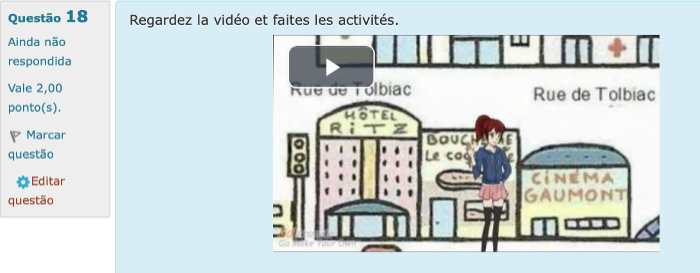
\includegraphics[width=\textwidth]{imagem1.png}
		\caption{Seção \textit{Étude du genre textuel.}}
		\label{fig-1}
		\source{Elaboração própria}
	\end{minipage}
\end{figure}


Nestas duas primeiras etapas, nosso objetivo era desenvolver as
capacidades de ação, por meio da construção de sentido a partir de
representações dos elementos do contexto de produção, da mobilização dos
conteúdos e da escolha do gênero textual \cite{bronckart_atividade_1999}. Dessa
maneira, a fim de mobilizarmos os conhecimentos descritos e atingir de
maneira satisfatória o objetivo da atividade, utilizamos algumas das
funcionalidades oferecidas pela plataforma Moodle. Como se sabe, o
Moodle organiza suas ferramentas em duas categorias: atividades e
recursos. Para o exercício apresentado, foi escolhida a atividade
\enquote{Questionário}, ou seja, um conjunto de questões de vários formatos
diferentes. A ferramenta em questão, bastante utilizada na elaboração do
curso, permite a criação pelo professor de questões de vários formatos,
cabendo ao aluno escolher suas respostas e, em seguida, observar a
correção efetuada pelo sistema a partir de um gabarito previamente
inserido na plataforma pelo professor. No exercício elaborado, a
tipologia de atividade escolhida na plataforma se denomina \enquote{múltipla
escolha}, que permite, também, que o aluno faça mais de uma escolha e
que cada uma das tentativas seja corrigida imediatamente pelo Moodle. Já
o vídeo escolhido para a atividade foi retirado da plataforma YouTube e
inserido no Moodle por meio do recurso \enquote{Rótulo}, que permite a
inserção de textos, imagens e vídeos.

Na terceira subseção, intitulada \emph{focus langue}, buscamos mobilizar
tanto as capacidades discursivas quanto as capacidades
linguístico-discursivas relativas ao gênero textual diálogo. No que diz
respeito às capacidades discursivas, buscamos levar os alunos, por meio
de atividades variadas, a refletirem sobre aspectos organizacionais e
discursivos do gênero, como os tipos de sequência presentes e suas
relações com a situação de produção e os conteúdos temáticos veiculados.
Neste momento, nossa intenção era fazer com que os alunos refletissem
sobre a planificação global do texto, os segmentos organizados de forma
linguística no texto e suas formas de planificação, ou seja, as
sequências \cite{adam_1992,bronckart_atividade_1999}. Algumas de nossas preocupações eram fazer com que os alunos reconhecessem a organização do gênero a partir de seu planejamento geral e compreendessem a função da
organização do conteúdo no gênero diálogo, como ilustra o exercício a
seguir, previsto para que os alunos respondessem às perguntas que já
estavam dadas, relativas ao objetivo comunicativo de indicar um
itinerário na rua. Por meio deste exercício \Cref{fig-2}, os alunos
puderam perceber a forma de organização do conteúdo mobilizado e
refletir sobre a organização do texto.


\begin{figure}[htbp]
	\centering
	\begin{minipage}{0.8\textwidth}
		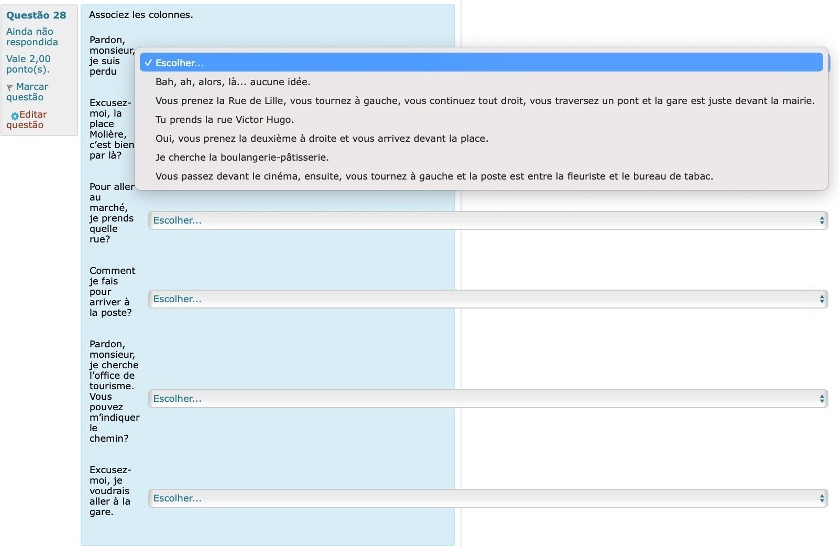
\includegraphics[width=\textwidth]{imagem2.png}
		%Extraído como InkScape
		\caption{Seção \textit{Focus langue.}}
		\label{fig-2}
		\source{Elaboração própria}
	\end{minipage}
\end{figure}

Em relação às capacidades linguístico-discursivas, o objetivo principal
era que os alunos refletissem sobre o estudo da língua francesa, que
elaborassem uma reflexão sobre os elementos linguísticos característicos
do gênero diálogo a partir de uma proposta que partiria da observação à
sistematização da regra. A gramática, neste material, foi considerada
como uma atividade heurística, que permitia ao aluno a reflexão sobre a
língua e a construção de um saber organizado sobre seu funcionamento.
Dessa forma, diferentemente da maioria dos cursos propostos para o
ensino de FLE, os alunos, por meio do método indutivo e mediante a
exposição ao corpus linguístico e a observação de exemplos, puderam
construir as regras e compreender os princípios gramaticais da língua
francesa, o que contribuiu possivelmente para a valorização da
descoberta de regras e das generalizações necessárias naquele estágio,
como comprovaram as produções orais e escritas entregues aos estagiários
para correção.

No exemplo apresentado \Cref{fig-3}, o objetivo é aprender a conjugação do
verbo \emph{prendre} (\enquote{pegar}, \enquote{tomar}), no presente do Indicativo, para, em um contexto de indicar o itinerário na rua, ser capaz de
utilizar, de maneira autônoma, as expressões linguísticas adequadas a
esse fim. A plataforma Moodle permitiu à equipe, também por meio da
ferramenta \enquote{atividades} e \enquote{questionário}, construir de forma
indutiva, como explicado, um exercício por meio da funcionalidade
\enquote{arrastar e soltar na imagem}, em que caberá ao aluno escolher a forma
verbal correspondente, proposta na parte inferior da imagem e, clicando
sobre a forma escolhida, arrastá-la com o mouse até o espaço que
contempla sua resposta. Assim como no exercício descrito anteriormente,
múltiplas respostas são consideradas, mas apenas uma, corrigida
imediatamente pela plataforma Moodle, é considerada adequada.

\begin{figure}[htbp]
	\centering
	\begin{minipage}{0.8\textwidth}
		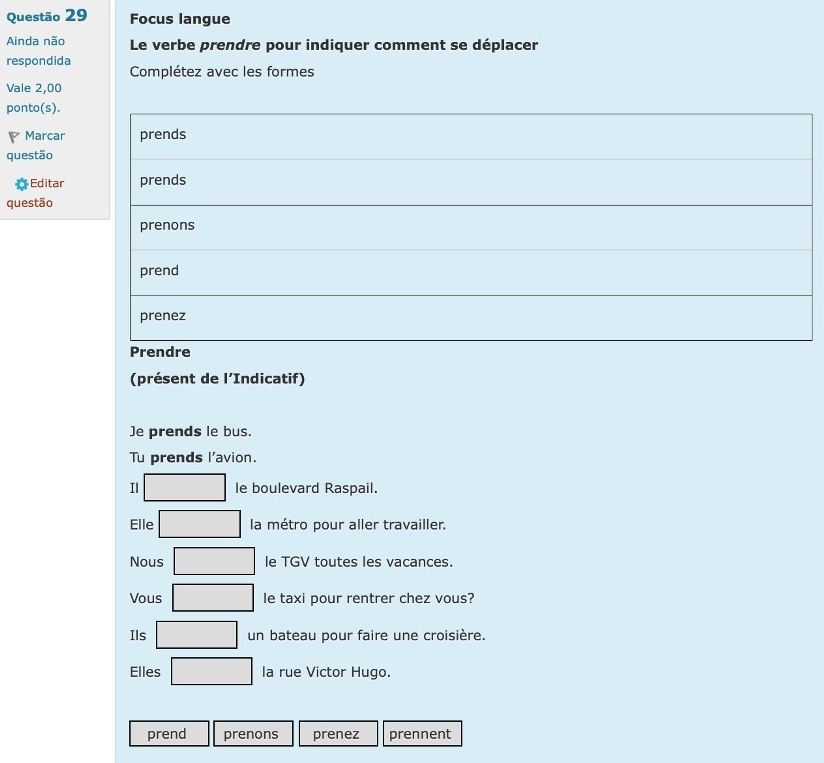
\includegraphics[width=\textwidth]{imagem3.png}
		%Extraído com o InkScape
		\caption{Seção \emph{Focus langue}}
		\label{fig-3}
		\source{Elaboração própria}
	\end{minipage}
\end{figure}


A quarta e última atividade que apresentaremos da lição 3 diz respeito a
uma das propostas de produção oral, sempre associadas ao gênero textual
proposto como texto autêntico de partida para a unidade, ou seja, o
diálogo. A ideia principal, neste momento, é inserir o estudante em uma
situação de comunicação autêntica, o que lhe permite adaptar-se a
situações concretas de uso da linguagem em um contexto francófono,
produzir um novo exemplar do gênero textual e mostrar o que efetivamente
aprendeu após ter realizado as atividades propostas.

Nas três unidades elaboradas, as propostas de produção oral e de
produção escrita permitiram a mobilização das três capacidades de
linguagem juntas, auxiliando, assim, os alunos a desenvolverem não só o
capital linguístico adquirido até então, mas também estratégias de
produção que os conduziam à autonomia em francês. As tarefas de produção
que refletiam situações autênticas em diferentes domínios sociais
(pessoal, público, profissional, etc.) podem ser ilustradas pelo
exercício da \Cref{fig-4}.

\begin{figure}[htbp]
	\centering
	\begin{minipage}{0.8\textwidth}
		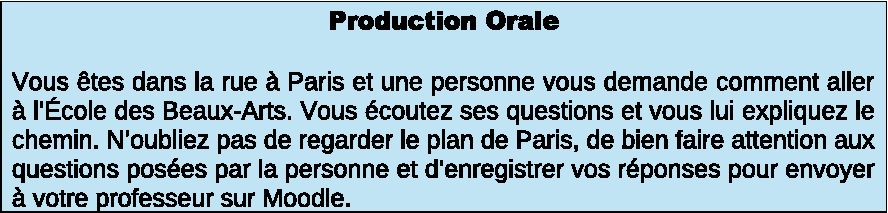
\includegraphics[width=\textwidth]{imagem4.pdf}
		%extraída usando o InkScape
		\caption{Seção Produção Oral}
		\label{fig-4}
		\source{Elaboração própria}
	\end{minipage}
\end{figure}

Como as aulas eram totalmente assíncronas, as atividades de produção
oral foram adaptadas para refletirem o máximo possível a interação
autêntica em contexto, buscando superar, por vezes, a falta de
espontaneidade decorrente desta modalidade de trabalho. A partir das
explicações no enunciado do exercício, o aluno deveria, inicialmente,
observar um mapa de Paris inserido na plataforma Moodle. Neste mapa,
além da imagem de uma parte da cidade, com suas ruas, pontes,
monumentos, comércios, etc, havia a imagem de duas pessoas que simulavam
um diálogo em uma das ruas. No contexto preparado, uma das pessoas
julgava estar perdida e pedia a outra que lhe explicasse como chegar à
\emph{École des Beaux-Arts} (\enquote{Escola de Belas-Artes}). Ao aluno, no
diálogo, caberia explicar o itinerário, cumprindo, assim, um dos
objetivos comunicativos da lição. Era necessário, portanto, observar o
mapa para se localizar, escutar as frases da pessoa que pedia a
informação (já gravadas pelos estagiários e disponibilizadas no Moodle
em arquivo mp3) e responder a elas, indicando o itinerário demandado a
partir do mapa, buscando simular um diálogo o mais natural possível.
Todas as frases já gravadas pelos estagiários apresentavam, ao seu
final, um sinal sonoro, que indicava o momento em que os alunos deveriam
começar a produzir as suas falas. As falas gravadas pelos alunos, que
completavam o diálogo a partir das frases já gravadas, deveriam ser
enviadas por meio da ferramenta \enquote{Arquivo} da plataforma Moodle, para
que as devidas correções fossem efetuadas pelos estagiários. Após a
correção, um retorno sobre a produção, avaliada em critérios de
adequação ao gênero textual, escolha e pertinência das ideias e dos
argumentos, organização dos conteúdos, coerência e coesão, sintaxe e
vocabulário foi disponibilizado na própria plataforma Moodle, de forma
que o aluno pudesse ter a correção comentada de seu texto e,
principalmente, a possibilidade de autocorreção futura.

Ainda que tenhamos destacado apenas quatro atividades, muitas outras
ferramentas disponibilizadas por Moodle foram igualmente utilizadas pela
equipe, entre elas: a ferramenta \enquote{Fórum}, momento em que uma discussão
assíncrona entre os alunos integrantes da disciplina e também entre
alunos e equipe de professores, sobre conteúdos ministrados, foi
proposta pela equipe; a ferramenta \enquote{Glossário}, em que a inclusão de
palavras pertencentes ao vocabulário relativo ao tema da unidade foi
efetuada; o recurso \enquote{inserir URL}, para que os integrantes da
disciplina pudessem assistir a vídeos oriundos de outras plataformas e
desenvolver sua compreensão oral.

Na última seção, apresentaremos algumas reflexões à guisa de conclusão.

\section{Considerações finais}

Neste texto, buscamos apresentar e descrever parte de um processo de elaboração de um material didático para um curso de FLE, assíncrono, realizado por meio da plataforma Moodle, organizado pelo viés dos gêneros textuais. Nosso intuito foi mostrar como o material em questão, ancorado teoricamente pelo ISD, foi pertinente ao apresentar diversas atividades para o aprendizado do francês, em seu nível inicial, além de propiciar o desenvolvimento das capacidades de linguagem dos alunos, capacidades essas que são transferíveis a outros gêneros textuais que futuramente serão produzidos pelos alunos nas mais diversas situações do agir social. Isso mostra a relevância do trabalho com gêneros textuais no ensino de línguas, uma vez que o aprendizado não se concentra apenas no gênero estudado, ou seja, no trabalho do “gênero pelo gênero”, que cataloga a descrição de cada estilo, de cada estrutura composicional e de cada conteúdo temático, mas naquilo, principalmente, que o gênero é capaz de desenvolver em termos de capacidades, auxiliando o aluno a melhor ler, escutar, escrever e falar numa dada situação de comunicação.

Dessa forma, interpretando o trabalho realizado, podemos afirmar que o curso efetuou, de maneira satisfatória, a transposição didática dos conceitos propostos pelo ISD para as atividades desenvolvidas, embora nem todos os gêneros propostos para atividades de produção oral e produção escrita tenham sido ensinados a partir de um modelo didático o mais completo possível, como apregoa a teoria. Em virtude da falta de tempo, muitas dessas atividades foram elaboradas a partir de um modelo didático mais simples, mas que, no entanto, não deixou de cumprir o mínimo possível em termos de mapeamento das principais características dos gêneros. O grau de domínio dos conhecimentos teóricos pelo professor-supervisor auxiliou consideravelmente os estagiários no trabalho, o que podemos considerar também um aspecto também de formação.

Em relação à participação da equipe de estagiários, é válido destacar seu engajamento e sua preocupação em desenvolver atividades as mais diversificadas possíveis dentro do que a plataforma Moodle poderia oferecer no momento, o que, certamente, possibilitará aos alunos inscritos no curso a oportunidade de acessar as noções trabalhadas para o ensino da língua francesa de diversas maneiras distintas, no seu tempo e no seu estágio de aprendizado, garantindo, assim, as chances de êxito.

Finalmente, quanto ao trabalho de formação realizado, julgamos que o trabalho foi exitoso, na medida em que implicou os próprios estagiários na construção de seu material didático, experiência bastante rara no ensino de línguas, abrindo-se ao diálogo e à escuta do outro, em uma análise crítica do seu próprio trabalho e do seu desenvolvimento enquanto futuro professor de francês. Resta-nos, agora, analisar o resultado concreto do aprendizado junto aos matriculados no curso, o que possibilitará uma avaliação mais ampla e completa da experiência.


\printbibliography\label{sec-bib}

\end{document}
